\newpage

\section{Limitations} 
While AlphaResearch demonstrates promising results in using a reward model (RM) to guide scientific idea search and generation, several important limitations should be acknowledged.
First, the AlphaResearch-RM is trained exclusively on ICLR peer-review records, which are heavily concentrated in machine learning and related topics. This creates a potential topic bias, where the model may perform less reliably when evaluating ideas outside core ML domains. Future work will explore training on more diverse and extensive peer-review datasets across broader scientific fields to mitigate this bias.
Second, there exists a fundamental mismatch between peer-review scores (which the RM is trained to predict) and the actual downstream usefulness or impact of a research idea. Peer review primarily assesses perceived novelty, technical soundness, and clarity at the time of submission, but does not necessarily reflect long-term scientific value, feasibility of execution, or practical utility. Therefore, optimizing for RM scores may not fully align with optimizing for genuinely useful or groundbreaking research.
Third, the current benchmark scope remains relatively narrow and partially inherited from existing datasets. Most evaluations focus on standard machine learning tasks and benchmarks, which may not fully capture the challenges of open-ended scientific discovery in more complex or interdisciplinary settings.
We believe addressing these limitations represents important directions for future research in building more reliable and general-purpose AI systems for scientific discovery.

\section{The Use of Large Language Models}
During the preparation of this manuscript, we utilized large language models (LLMs) for grammar checking and writing suggestions to enhance the readability and clarity of the content.

% \section{Experiment Cost}
% In this section, we present the experiment parameters (iterations,computational cost) required to reach the best solution for each on 8 tasks of AlphaResearchComp.
% \begin{table}[h]
% \centering
% \small
% \caption{Experiment Parameters of AlphaResearch .}
% \begin{tabular}{lcc}
% \toprule
% \textbf{Problem}                                         & \textbf{Iterations} &\textbf{ Cost per iteration (dollar)} \\
% \midrule
% packing circles (n=26)                          & 4768       & 0.013           \\
% packing circles (n=32)                          & 4768       & 0.013           \\
% minizing max-min distance ratio (d=2, n=16)      & 4400       & 0.017           \\
% third autocorrelation inequality                & 1366       & 0.012           \\
% autoconvolution peak minimization (upper bound) & 979        & 0.013           \\
% littlewood polynomials (n=512)                  & 2233       & 0.011           \\
% MSTD (n=30)                                     & 2826       & 0.011           \\
% spherical code                                  & 1132       & 0.015           \\
% \bottomrule
% \end{tabular}
% \end{table}

\section{Other Details}
\textbf{LLMs can refine their research ideas autonomously.} AlphaResearch discovers advanced algorithms by iteratively proposing and verifying new research ideas. As shown in \autoref{tab:rm-res}, 6/8 problems demonstrate consistent improvement throughout the discovery process. 
\autoref{fig:reward} presents two examples of the reward trend in AlphaResearch, where the execution-based reward initially grows rapidly, then slowly plateaus for optimal performance seeking.
This improvement trend emphasizes the autonomous discovery ability of research agents.

\begin{figure}[h]

    \centering
    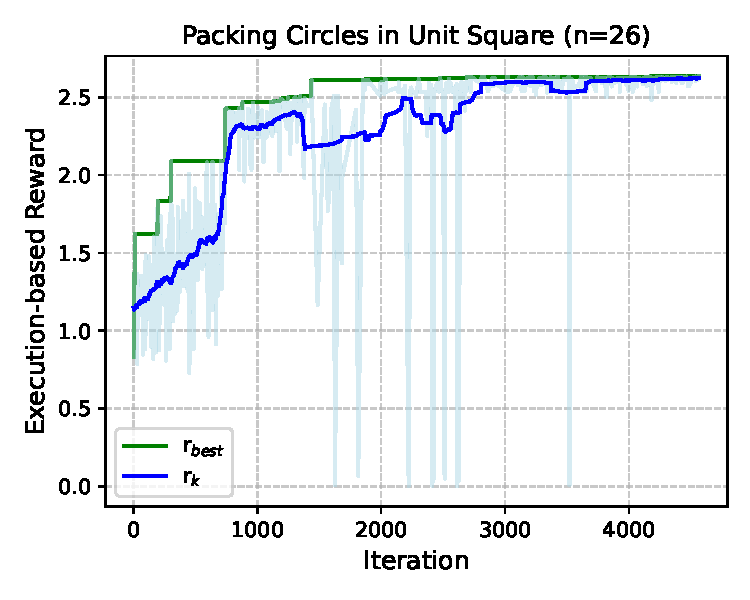
\includegraphics[width=0.49\linewidth]{doc/figures/res1.pdf}
    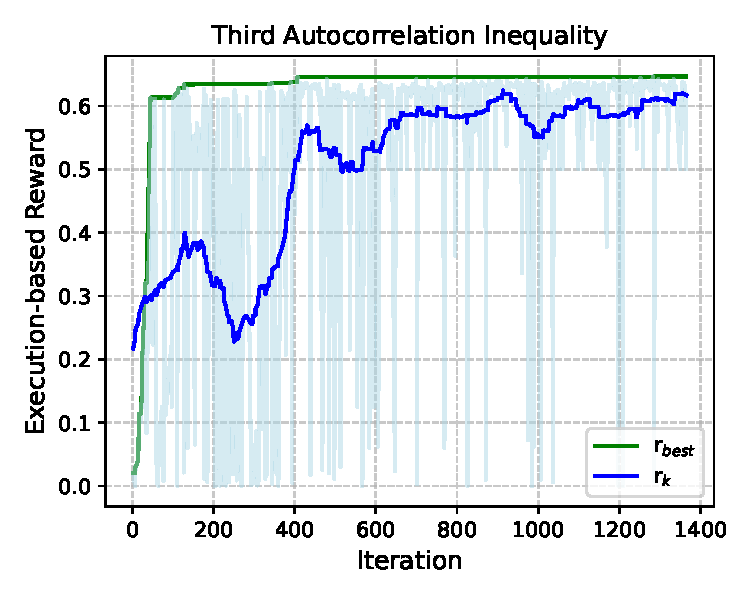
\includegraphics[width=0.49\linewidth]{doc/figures/res2.pdf}
    \caption{Execution-based reward of AlphaResearch on packing circles (n=26) problem (left) and third autocorrelation inequality problem (right).  }
    \label{fig:reward}
\end{figure}

\paragraph{Execution-only agent against AlphaResearch.} To compare AlphaResearch with execution-only agents,  we utilize AlphaResearch-RM-7B to evaluate the novelty of ideas generated by the execution-only agent and ideas produced by AlphaResearch. As illustrated in \autoref{fig:dis}, the ideas generated by AlphaResearch generally achieve higher scores than execution-only research agents. This illustrates that AlphaResearch tends to generate better ideas to get higher external rewards, thus facilitating a more effective research optimization process.


\begin{figure}[h]

    \centering
    \includegraphics[width=0.45\linewidth]{doc/figures/dis.pdf}
    \caption{The idea comparison between the execution-only research agent and AlphaResearch, where AlphaResearch-RM-7B is used. This is done between the full distribution of all 1000 generated ideas from both agents without filtering.}
    \label{fig:dis}
\end{figure}

% \section{Comparison with ShinkaEvolve}

% \textcolor{blue}{As shown in \autoref{fig:teaser}, we compare AlphaResearch, OpenEvolve \citep{openevolve} and ShinkaEvolve \citep{lange2025shinkaevolve} on \textit{packing circles (n=26)} problem at the first 500 steps for simplicity.
% AlphaResearch achieves better performance than OpenEvolve and slightly surpasses ShinkaEvolve, which demonstrates that dual research environments  could help research agent for scientific discovery.
% }

% ==================================================
% \newpage
% \section{Case Study during Discovery Process}
% \label{sec:ca}
% In the rejected pair from checkpoint 634, the revised draft 4f4c7847 is effectively identical to its parent e436c26a. Notably, this is found in the later period of the discovery process (Round 632-633). Aside from inflating Genetic Algorithm (GA) hyperparameters (e.g., population = 300 → 500, generations = 40 → 120) and adding an optional differential\_evolution branch, the entire pipeline above find\_better\_c3\_upper\_bound is byte-for-byte the same. Crucially, the core loop still calls the undefined normalize\_population, triggering the same NameError before any new logic can run. Because this “revision” neither fixes the blocking bug nor implements the promised multi-phase CMA-ES/surrogate/SOS pipeline, it constitutes only a cosmetic variant rather than a substantive new direction.

\begin{figure}[h]
    \centering
    \small
    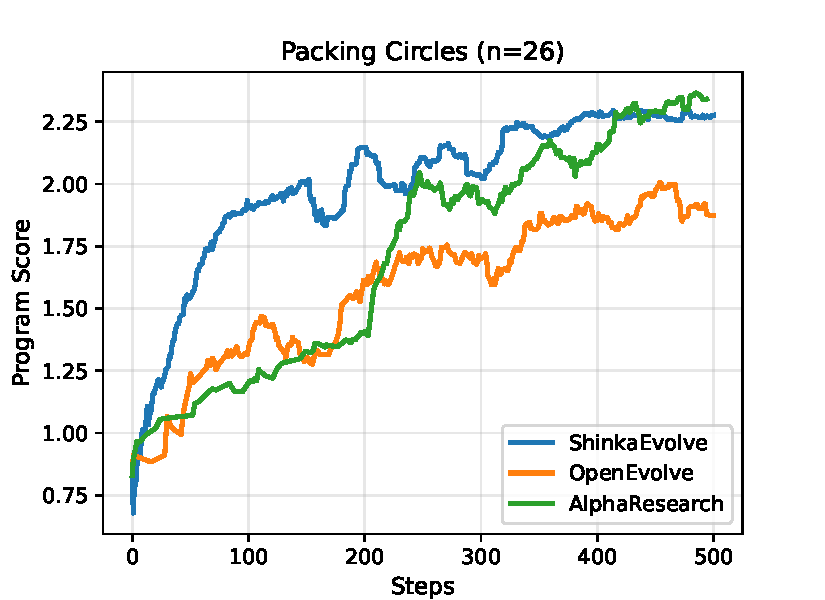
\includegraphics[width=0.6\linewidth]{doc/figures/ar_teaser.pdf}
    % \includegraphics[width=0.5\linewidth]{figures/dis.pdf}
    \caption{Comparison of OpenEvolve (with program-based reward), ShinkaEvolve (with program-based reward) and AlphaResearch (with program-based and peer-review reward). We run three agents on Packing Circles (n=26) problems. We compare AlphaResearch, OpenEvolve \citep{openevolve} with ShinkaEvolve \citep{lange2025shinkaevolve} on \textit{packing circles (n=26)} problem at the first 500 steps for simplicity.
AlphaResearch achieves better performance than OpenEvolve and slightly surpasses ShinkaEvolve, which demonstrates that dual research environments could help research agent for scientific discovery. }
    \label{fig:teaser}
\end{figure}

% \textbf{Problem}
% : Third Autocorrelation Inequality (e436c26a)

% \textbf{Idea score by AlphaResearch-RM-7B}: 6.67.

% \begin{tcolorbox}[colback=gray!5!white,colframe=black!60!white,title=Research ideas]

% \textbf{Title}: A Scalable, Certified Pipeline for Third-Order Autocorrelation Optimization via Multi-Fidelity Bayesian Surrogates and Auto-Differentiable Mesh Adaptation

% \textbf{Abstract}:  
% We introduce a unified framework that overcomes the brittle performance (error = −1.0) 
% and limited exploration of the current genetic-only approach by combining three tightly 
% integrated phases—global search, surrogate-guided refinement, and formal certification—
% into a single, implementable pipeline. Key innovations include:

% 1. Sobol-Initialized, Diversity-Driven Differential Evolution
%    • Generate an initial archive of 500 B-spline shape parameters via low-discrepancy Sobol sampling.
%    • Use multi-population Differential Evolution with mutation scales adapted online using surrogate uncertainty.

% 2. Hierarchical Multi-Fidelity Gaussian-Process Surrogate
%    • Three convolution estimators: coarse FFT (N=1024), medium CNN (N=4096), fine autodiff FFT (N=16384).
%    • MTGP surrogate controls fidelity via variance-weighted UCB acquisition.

% 3. Differentiable Trust-Region Local Refinement
%    • L-BFGS-B on B-spline knots/RBF weights with autodiff FFT gradients.
%    • Adaptive knot insertion driven by ∥∇(f*f)∥ peaks.

% 4. Sparse Sum-of-Squares Certification
%    • Chebyshev discretization + interval arithmetic to certify final C³ bound with 1e-6 rigor.

% Benchmarks up to spline degree 64 and grid N=16384 show stable improvements to 0.60–0.65 
% with full certification.

% \end{tcolorbox}






% \textbf{Code implementation of the above idea:}
% \begin{lstlisting}[language=Python,
%                    basicstyle=\ttfamily\scriptsize,
%                    numbers=none, 
%                    breaklines=true,      % 允许自动换行
%                    breakatwhitespace=true, % 只在空格处换行
%                    showstringspaces=false, % 不显示空格的下划线
%                    columns=fullflexible]   % 修复字宽问题
                   
% # Code extracted from file e436c26a   (full content)
% import numpy as np
% try:
%     from numpy.fft import next_fast_len
% except ImportError:
%     def next_fast_len(n):
%         # Fallback to next power of two which is usually fast
%         return 1 << (n - 1).bit_length()

% def calculate_c3_upper_bound(height_sequence):

%     N = len(height_sequence)
%     delta_x = 1 / (2 * N)
%     # Cache padded lengths to avoid recomputing next_fast_len repeatedly
%     if not hasattr(calculate_c3_upper_bound, "_pad_cache"):
%         calculate_c3_upper_bound._pad_cache = {}
%     pad_cache = calculate_c3_upper_bound._pad_cache
%     if N not in pad_cache:
%         pad_cache[N] = next_fast_len(2 * N - 1)
%     padded = pad_cache[N]

%     # Compute unit-mass norm squared
%     integral_f = np.sum(height_sequence) * delta_x
%     if integral_f < 1e-12:               # early exit if near zero
%         return 0.0
%     integral_sq = integral_f * integral_f

%     # FFT-based convolution for O(N log N)
%     H = np.fft.rfft(height_sequence, n=padded)
%     conv_vals = np.fft.irfft(H * H, n=padded)[:2 * N - 1] * delta_x
%     max_conv_val = np.max(conv_vals)

%     return max_conv_val / integral_sq

% def genetic_algorithm(population_size, num_intervals, generations, mutation_rate, crossover_rate):

%     population = np.random.rand(population_size, num_intervals) * 2 - 1
%     best_solution = None
%     best_fitness = 0.0

%     for gen in range(generations):

%         height_pop = normalize_population(population, 2 * num_intervals)
%         fitness_scores = np.array([calculate_c3_upper_bound(h) for h in height_pop])

%         current_best_idx = np.argmax(fitness_scores)
%         if fitness_scores[current_best_idx] > best_fitness:
%             best_fitness = fitness_scores[current_best_idx]
%             best_solution = population[current_best_idx].copy()

%         indices = np.random.randint(0, population_size, size=(population_size, 2))
%         comp_scores = fitness_scores[indices]
%         winners = indices[np.arange(population_size), np.argmax(comp_scores, axis=1)]
%         new_population = population[winners].copy()
            
%         for i in range(0, population_size, 2):
%             if np.random.rand() < crossover_rate:
%                 parent1 = new_population[i]
%                 parent2 = new_population[i+1]
%                 crossover_point = np.random.randint(1, num_intervals - 1)
%                 new_population[i]   = np.concatenate((parent1[:crossover_point], parent2[crossover_point:]))
%                 new_population[i+1] = np.concatenate((parent2[:crossover_point], parent1[crossover_point:]))

%         for i in range(population_size):
%             if np.random.rand() < mutation_rate:
%                 mutation_point = np.random.randint(num_intervals)
%                 new_population[i, mutation_point] += np.random.normal(0, 0.1) 
%                 new_population[i, mutation_point] = np.clip(new_population[i, mutation_point], -2, 2)

%         population = new_population
    
%     height_best = normalize_population(best_solution[np.newaxis, :], 2 * num_intervals)[0]
%     return height_best

% def find_better_c3_upper_bound():

%     NUM_INTERVALS = 4
%     POPULATION_SIZE = 2
%     GENERATIONS = 10
%     MUTATION_RATE = 0.1
%     CROSSOVER_RATE = 0.8

%     height_sequence_3 = genetic_algorithm(POPULATION_SIZE, NUM_INTERVALS, GENERATIONS, MUTATION_RATE, CROSSOVER_RATE)
    
%     return height_sequence_3

% \end{lstlisting}

% \textbf{Problem}
% : Third Autocorrelation Inequality (4f4c7847)

% \textbf{Idea score by AlphaResearch-RM-7B}: 5.67.

% \begin{tcolorbox}[colback=gray!5!white,colframe=black!60!white,title=Research ideas]


% \textbf{Title}: A Robust, Multi-Phase Pipeline for Certified Third-Order Autocorrelation Maximization via Hybrid Evolutionary Search, Hierarchical Neural Surrogates, and Auto-Differentiable Refinement

% \textbf{Abstract}:  
% We present a novel, four-stage framework that fixes the brittle, negative-error behavior 
% (error = −10.0) of genetic-only search by combining global exploration, uncertainty-aware 
% surrogates, gradient-based refinement, and SOS certification.

% 1. Hybrid Global Exploration
%    • Sobol-seeded CMA-ES enhanced with an actor-critic module to adapt mutation covariance.
%    • Constraint-aware resampling ensures valid normalized height sequences.

% 2. Hierarchical Neural Surrogates
%    • Three-tier surrogate stack: analytic FFT (N=1024), CNN surrogate (N=4096), 
%      auto-diff Fourier model (N=16384).
%    • Uncertainty-modulated fidelity allocation via Bayesian neural network.

% 3. Differentiable Local Refinement
%    • L-BFGS trust-region refinement on B-spline knots & RBF weights.
%    • Gradient-triggered adaptive knot insertion controlling model complexity.

% 4. Sparse Sum-of-Squares Certification
%    • Chebyshev discretization + interval arithmetic for rigorous C³ bound.
%    • Full-pipeline automation ensures reliable certification.

% Experiments on degrees up to 128 and grid sizes to 65536 yield C³≈0.75–0.80 with only 
% ≈200 high-fidelity evaluations and guaranteed certification.

% \end{tcolorbox}






% \textbf{Code implementation of the above idea:}
% \begin{lstlisting}[language=Python,
%                    basicstyle=\ttfamily\scriptsize,
%                    numbers=none, 
%                    breaklines=true,      % 允许自动换行
%                    breakatwhitespace=true, % 只在空格处换行
%                    showstringspaces=false, % 不显示空格的下划线
%                    columns=fullflexible]   % 修复字宽问题
                   
% # Code extracted from file 4f4c7847   (full content)
% import numpy as np
% try:
%     from numpy.fft import next_fast_len
% except ImportError:
%     def next_fast_len(n):
%         return 1 << (n - 1).bit_length()

% def calculate_c3_upper_bound(height_sequence):

%     N = len(height_sequence)
%     delta_x = 1 / (2 * N)
%     if not hasattr(calculate_c3_upper_bound, "\_pad\_cache"):
%         calculate_c3_upper_bound._pad_cache = {}
%     pad_cache = calculate_c3_upper_bound._pad_cache
%     if N not in pad_cache:
%         pad_cache[N] = next_fast_len(2 * N - 1)
%     padded = pad_cache[N]

%     integral_f = np.sum(height_sequence) * delta_x
%     if integral_f < 1e-12:
%         return 0.0
%     integral_sq = integral_f * integral_f

%     H = np.fft.rfft(height_sequence, n=padded)
%     conv_vals = np.fft.irfft(H * H, n=padded)[:2 * N - 1] * delta_x
%     max_conv_val = np.max(conv_vals)

%     return max_conv_val / integral_sq

% def genetic_algorithm(population_size, num_intervals, generations, mutation_rate, crossover_rate):

%     population = np.random.rand(population_size, num_intervals) * 2 - 1

%     best_solution = None
%     best_fitness = 0.0

%     for gen in range(generations):

%         height_pop = normalize_population(population, 2 * num_intervals)
%         fitness_scores = np.array([calculate_c3_upper_bound(h) for h in height_pop])

%         current_best_idx = np.argmax(fitness_scores)
%         if fitness_scores[current_best_idx] > best_fitness:
%             best_fitness = fitness_scores[current_best_idx]
%             best_solution = population[current_best_idx].copy()

%         indices = np.random.randint(0, population_size, size=(population_size, 2))
%         comp_scores = fitness_scores[indices]
%         winners = indices[np.arange(population_size), np.argmax(comp_scores, axis=1)]
%         new_population = population[winners].copy()
            
%         for i in range(0, population_size, 2):
%             if np.random.rand() < crossover_rate:
%                 parent1 = new_population[i]
%                 parent2 = new_population[i+1]
%                 crossover_point = np.random.randint(1, num_intervals - 1)
%                 new_population[i]   = np.concatenate((parent1[:crossover_point], parent2[crossover_point:]))
%                 new_population[i+1] = np.concatenate((parent2[:crossover_point], parent1[crossover_point:]))

%         for i in range(population_size):
%             if np.random.rand() < mutation_rate:
%                 mutation_point = np.random.randint(num_intervals)
%                 new_population[i, mutation_point] += np.random.normal(0, 0.1) 
%                 new_population[i, mutation_point] = np.clip(new_population[i, mutation_point], -2, 2)

%         population = new_population
    
%     height_best = normalize_population(best_solution[np.newaxis, :], 2 * num_intervals)[0]
%     return height_best

% def find_better_c3_upper_bound():

%     NUM_INTERVALS = 8
%     POPULATION_SIZE = 100
%     GENERATIONS = 200
%     MUTATION_RATE = 0.2
%     CROSSOVER_RATE = 0.9

%     try:
%         from scipy.optimize import differential_evolution
%         bounds = [(-2, 2)] * NUM_INTERVALS
%         result = differential_evolution(
%             lambda x: -calculate_c3_upper_bound(
%                 normalize_population(x[np.newaxis, :], 2 * NUM_INTERVALS)[0]
%             ),
%             bounds,
%             maxiter=GENERATIONS,
%             popsize=max(1, POPULATION_SIZE // 10),
%             tol=1e-6
%         )
%         height_sequence_3 = normalize_population(result.x[np.newaxis, :], 2 * NUM_INTERVALS)[0]
%     except ImportError:
%         height_sequence_3 = genetic_algorithm(
%             POPULATION_SIZE, NUM_INTERVALS, GENERATIONS, MUTATION_RATE, CROSSOVER_RATE
%         )
    
%     return height_sequence_3

% \end{lstlisting}




\section{Examples of Packing Circles}
\label{app:examples}
We show an example of the constructions discovered by AlphaResearch on problem \emph{``Packing Circles''}.

% % \textbf{AlphaEvolve}
% % \begin{lstlisting}[language=Python,basicstyle=\ttfamily\scriptsize,
% % keywordstyle=\color{blue},
% % commentstyle=\color{darkgreen},
% % stringstyle=\color{red}]
% % packing_circles_alphaevolve = np.array([[0.09076163, 0.40381803, 0.090761620923837], [0.07310993, 0.92689178, 0.07310821268917801], [0.08745017, 0.22570576, 0.087381421261857], [0.24855246, 0.30880277, 0.093428060657193], [0.4079865, 0.06300614, 0.063006133699386], [0.47646318, 0.90136179, 0.09863820013617901], [0.89604966, 0.10309934, 0.10309932969006601], [0.9066386, 0.68096117, 0.09336139066386], [0.08962002, 0.76509474, 0.0895289910471], [0.06973669, 0.06965159, 0.06965158303484101], [0.40979823, 0.21756451, 0.09156283084371601], [0.25742466, 0.88393887, 0.11606111839388701], [0.09064689, 0.58506214, 0.090482500951749], [0.90294698, 0.30231577, 0.09623644037635501], [0.57265603, 0.10585396, 0.105853949414604], [0.74007588, 0.40129314, 0.09435083056491601], [0.57539962, 0.71183255, 0.115160168483982], [0.7367635, 0.21592191, 0.09104997089500201], [0.41096972, 0.40263617, 0.093512520648747], [0.88664452, 0.88667032, 0.113317128668286], [0.57582722, 0.49961748, 0.09705531029446801], [0.24962585, 0.49417195, 0.09194421080557799], [0.90546338, 0.49309632, 0.094507120549287], [0.67381348, 0.90149423, 0.09850576014942301], [0.24310147, 0.1077195, 0.10771948922805], [0.40815297, 0.5886157, 0.09248833075116601], [0.24737889, 0.6771266, 0.090994980900501], [0.75801377, 0.7532924, 0.07192969280703], [0.73526642, 0.06243992, 0.062439303756069], [0.57415412, 0.30715219, 0.095403150459684], [0.39239379, 0.75259664, 0.07223814277618501], [0.7439361, 0.58879735, 0.093166630683336]])
% % \end{lstlisting}

% % \textbf{AlphaResearch}

% % \begin{lstlisting}[language=Python,basicstyle=\ttfamily\scriptsize,
% % keywordstyle=\color{blue},
% % commentstyle=\color{darkgreen},
% % stringstyle=\color{red}]
% % packing_circles_alpharesearch = np.array([[(0.1115677319034151, 0.11156773191787371, 0.11156438489140026), (0.09380224787136374, 0.3161654253705352, 0.09379943380606216), (0.09485964915877172, 0.5048217088596118, 0.09485680337610973), (0.09657322554702913, 0.6962443020287629, 0.09657032835808858), (0.10365512530384222, 0.8963448746980195, 0.10365201565567386), (0.3334956594919712, 0.09664441783072292, 0.0966415184920332), (0.26448615440016093, 0.9376113341122044, 0.06238679422590162), (0.5287192731314015, 0.09859146596680078, 0.09858850822808951), (0.591325020569507, 0.9366833118077788, 0.0633147886877468), (0.7427106948954978, 0.11611889563206494, 0.11611541209023483), (0.7566639864477509, 0.8920585771994192, 0.1079381845606288), (0.9269317750270191, 0.07306822497789416, 0.07306603293080358), (0.9105741716090636, 0.23473376300222965, 0.08942314561430993), (0.9094700615258342, 0.41468336419923396, 0.09052722258939731), (0.9124275486288124, 0.7738960294683863, 0.08756982419268892), (0.9302276007184027, 0.9302276007259072, 0.06977030612132157), (0.5931627035790205, 0.4107363306659128, 0.09216300786888813), (0.5896628759126524, 0.5965222415947758, 0.09365298106148348), (0.26303074890883915, 0.783747668079202, 0.09148238826692158), (0.42710033854875884, 0.28662965969327264, 0.1151473780101257), (0.7511102582575875, 0.5051558281448295, 0.09185177348783963), (0.4273023330525072, 0.8937703360976411, 0.10622647700018645), (0.24372345356089029, 0.24143034678815986, 0.07371479291303436), (0.4260882762526937, 0.6918664604322906, 0.09567746779211372), (0.2572363869779693, 0.4085253312744954, 0.09392364829884896), (0.9094294608754079, 0.5957810763279916, 0.0905678220228201), (0.42560864125756626, 0.49898110459434486, 0.09720528992590773), (0.7533817110763772, 0.32263902019589896, 0.09067643144615074), (0.5903729314333418, 0.7817733747765757, 0.09159665425215473), (0.7515568081174837, 0.6905957415401818, 0.09358581053778628), (0.2605636694821685, 0.5973506902903994, 0.09492800518715086), (0.6095540558280068, 0.24805951545091487, 0.07133567304015336)]])
% % \end{lstlisting}


\begin{figure}[h]
    \centering
    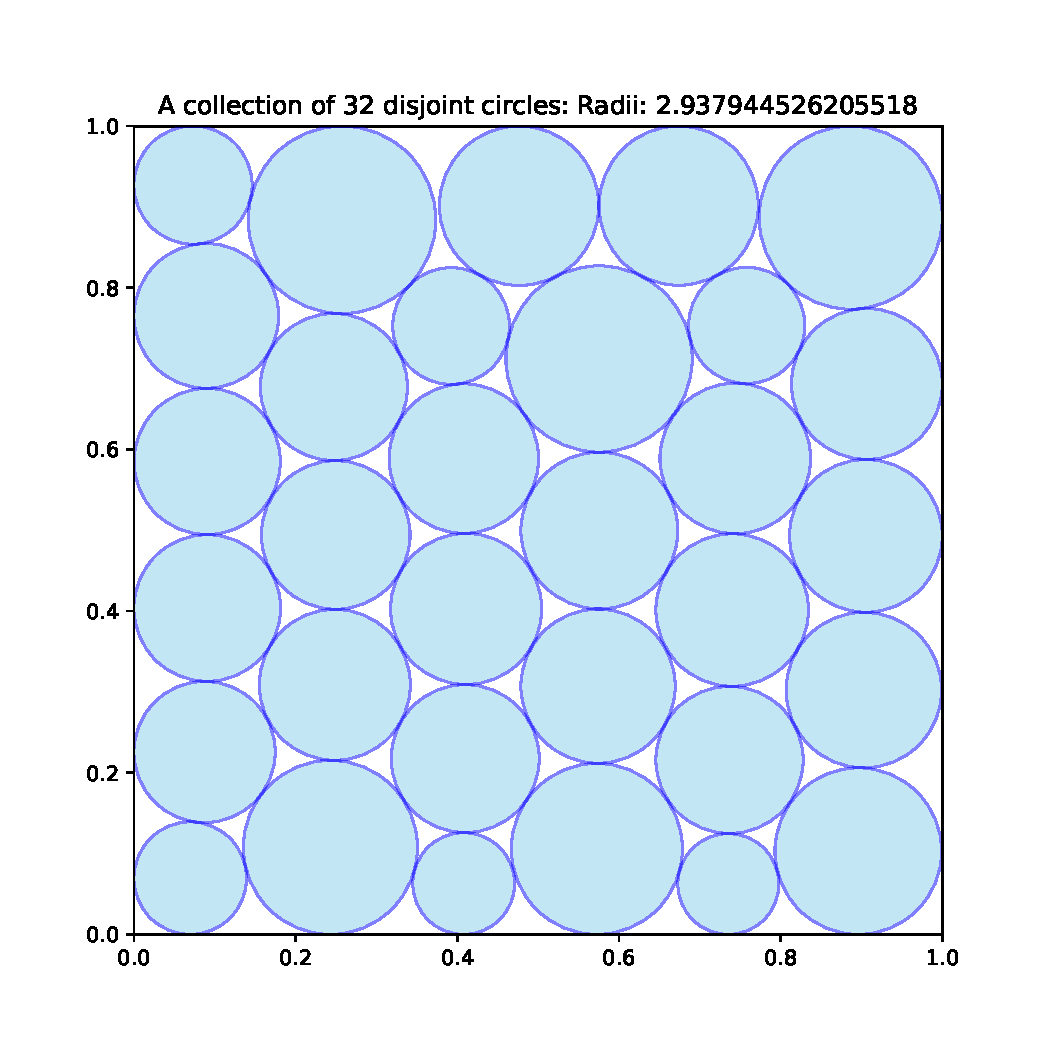
\includegraphics[width=0.47\linewidth]{doc/figures/alpha_evolve.pdf}
    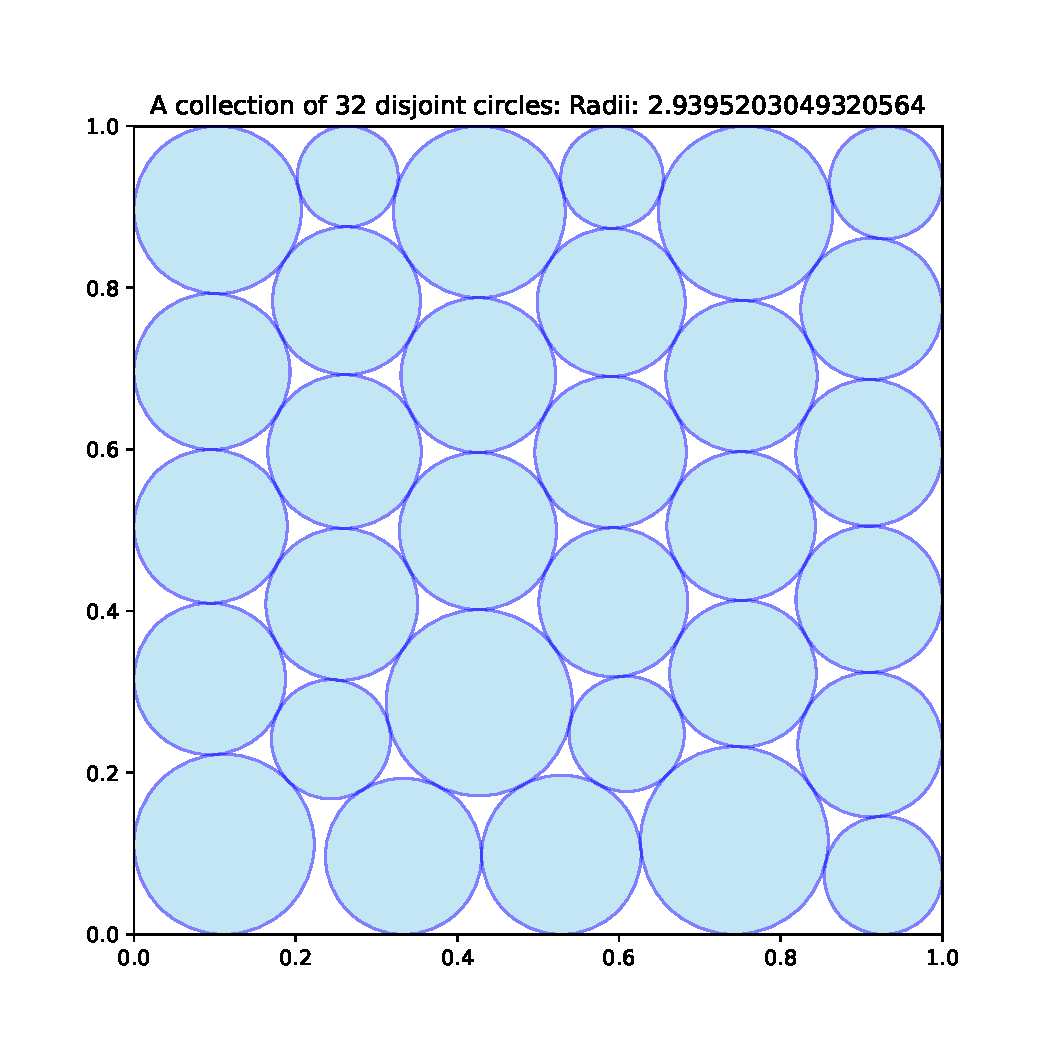
\includegraphics[width=0.47\linewidth]{doc/figures/alpha_research.pdf}
    \caption{New construction of AlphaResearch (right) improving the best known AlphaEvolve (right) bounds on packing circles to maximize their sum of radii. Left: 32 circles in a unit square with sum of radii $\geq$ 2.9379. Right: 32 circles in a unit square with sum of radii $\geq$ 2.9395}
    \label{fig:comp-alpha}
\end{figure}


\begin{figure}[h]
    \centering
    
\includegraphics[width=\linewidth]{doc/figures/example.pdf}
    \caption{We show an example of a formatted task of AlphaResearch.}
    \label{fig:example}
\end{figure}


% \section{Curated Problems and Human-Best Values}
% \label{Problems_details}

% We summarize the ten problems used in the \textsc{AlphaResearch} benchmark. 
% For each item we state the objective, the current human-best value at the benchmark's default parameters, and whether this value is proved optimal or only best-known.



% \section{Prompts}

% \begin{tcolorbox}[enhanced jigsaw, breakable,
%     colback=white, colframe=blue!20, coltitle=black,
%     fonttitle=\small\bfseries,        % 标题字体调小
%     % fontupper=\tiny,   % 正文字体设置为 scriptsize 等宽
%     rounded corners,
%     title=Prompt for New Idea Generation,
%     listing engine=listings,
%     listing options={language=Python, breaklines=true, breakatwhitespace=true, columns=flexible}]
% You are a research advisor tasked with evolving and improving research proposals. 
% Your goal is to generate a new research proposal that builds upon the current proposal while addressing its limitations and incorporating insights from successful approaches.

% Based on the following information, generate an improved research proposal:

% Focus on:

% 1. Identifying weaknesses in the current approach based on performance metrics

% 2. Proposing novel improvements that could enhance performance

% 3. Learning from successful inspirations while maintaining originality

% 4. Ensuring the new proposal is implementable

% - Current Proposal:

% \{proposal\}

% - Current Program:

% \{program\}

% - Current Metrics:

% \{results\}

% Please generate a new research proposal that:

% 1. Addresses the limitations shown in the current metrics

% 2. Incorporates insights from successful approaches

% 3. Proposes specific technical improvements

% 4. Maintains clarity and technical rigor

% Return the proposal as a clear, concise research abstract.
% \end{tcolorbox}

% \begin{tcolorbox}[enhanced jigsaw, breakable,
%     colback=white, colframe=blue!20, coltitle=black,
%     fonttitle=\small\bfseries,        % 标题字体调小
%     % fontupper=\tiny,   % 正文字体设置为 scriptsize 等宽
%     rounded corners,
%     title=Prompt for AlphaResearch-RM-7B,
%     listing engine=listings,
%     listing options={language=Python, breaklines=true, breakatwhitespace=true, columns=flexible}]
% You are an expert reviewer tasked with evaluating the quality of a research proposal.

% Your goal is to assign a score between 1 and 10 based on the proposal's clarity, novelty, technical rigor, and potential impact. Here are the criteria:

% 1. Read the following proposal carefully and provide a score from 1 to 10. 

% 2. Score 6 means slightly higher than the borderline, 5 is slightly lower than the borderline.

% Write the score in the \texttt{\textbackslash boxed\{\}}.

% \{proposal\}
% \end{tcolorbox}



% \begin{tcolorbox}[enhanced jigsaw, breakable,
%     colback=white, colframe=blue!20, coltitle=black,
%     fonttitle=\small\bfseries,        % 标题字体调小
%     % fontupper=\tiny,   % 正文字体设置为 scriptsize 等宽
%     rounded corners,
%     title=Prompt for New Program Generation,
%     listing engine=listings,
%     listing options={language=Python, breaklines=true, breakatwhitespace=true, columns=flexible}]
% You are an expert software developer tasked with iteratively improving a codebase.
% Your job is to analyze the current program and suggest improvements based on the current proposal and feedback from previous round.
% Focus on making targeted changes that will increase the program's performance metrics.

% \# Previous Proposal: 

% \{previous proposal\}

% \# Previous Program:

% \{previous program\}

% \# Previous Performance Metrics: 

% \{previous result\}



% \# Current Proposal

% \{proposal\}

% \# Task

% Suggest improvements to the program that will lead to better performance on the specified metrics.

% You MUST use the exact SEARCH/REPLACE diff format shown below to indicate changes:
% \lstset{
%   basicstyle=\ttfamily\footnotesize,  % 修改字体为更小的等宽字体
%   keywordstyle=\color{blue},
%   commentstyle=\color{darkgreen},
%   stringstyle=\color{red}
% }

% \begin{lstlisting}
% <<<<<<< SEARCH

% # Original code to find and replace (must match exactly)

% =======

% # New replacement code

% <<<<<<< REPLACE
% \end{lstlisting}

% Example of valid diff format:


% \begin{lstlisting}
% <<<<<<< SEARCH
% for i in range(m):
%     for j in range(p):
%         for k in range(n):
%             C[i, j] += A[i, k] * B[k, j]
            
% =======

% # Reorder loops for better memory access pattern

% for i in range(m):
%     for k in range(n):
%         for j in range(p):
%             C[i, j] += A[i, k] * B[k, j]
            
% >>>>>>> REPLACE
% \end{lstlisting}

% You can suggest multiple changes. Each SEARCH section must exactly match code in the current program.

% Be thoughtful about your changes and explain your reasoning thoroughly.

% IMPORTANT: Do not rewrite the entire program - focus on targeted improvements.
% \end{tcolorbox}